\documentclass[aspectratio=169,10pt,dvipsnames]{beamer} 
\usepackage{graphicx}
\usepackage{tabularx}
\usepackage{array}
\usepackage[most]{tcolorbox}
\usepackage{mathtools}
\usepackage{stackengine}
\usepackage{algorithmic}
\usepackage{epstopdf}
\usepackage{lipsum}
\usepackage{pifont}
\usepackage{algorithm}
\usepackage{tikz}
\usepackage{animate}
\usetikzlibrary{decorations.pathreplacing}
\usepackage[export]{adjustbox}
\renewcommand{\thealgorithm}{}
\usetikzlibrary{matrix}
\usepackage{natbib} 
\usepackage{bibentry}
\newcommand{\amin}{\mathop{\text{argmin}}}
\newcommand{\forestgreen}{\color{forestgreen}}
\newcommand{\red}{\color{red}}
\newcommand{\blue}{\color{blue}}
\newcommand{\bx}{\boldsymbol{x}}
\newcommand{\blambda}{\boldsymbol{\lambda}}
\newcommand{\by}{\boldsymbol{y}}
\newcommand{\bz}{\boldsymbol{z}}
\newcommand{\bX}{\boldsymbol{X}}
\newcommand{\bY}{\boldsymbol{Y}}
\newcommand{\bZ}{\boldsymbol{Z}}
\newcommand{\bv}{\boldsymbol{v}}
\newcommand{\bu}{\boldsymbol{u}}
\newcommand{\bxi}{\boldsymbol{\xi}}
\newcommand{\bpsi}{\boldsymbol{\psi}}
\newcommand{\bzeta}{\boldsymbol{\zeta}}
\newcommand{\boldsymbolu}{\boldsymbol{\mu}}
\newcommand{\bQ}{\boldsymbol{Q}}
\newcommand{\bS}{\boldsymbol{S}}
\newcommand{\bT}{\boldsymbol{T}}
\newcommand{\bF}{\boldsymbol{F}}
\newcommand{\bG}{\boldsymbol{G}}
\newcommand{\bd}{\boldsymbol{d}}
\newcommand{\bp}{\boldsymbol{p}}
\newcommand{\bff}{\boldsymbol{f}}
\newcommand{\bc}{\boldsymbol{c}}
\newcommand{\bg}{\boldsymbol{g}}
\newcommand{\bA}{\boldsymbol{A}}
\newcommand{\bB}{\boldsymbol{B}}
\newcommand{\bSigma}{\boldsymbol{\Sigma}}
\newcommand{\bC}{\boldsymbol{C}}
\newcommand{\bE}{\boldsymbol{E}}
\newcommand{\bh}{{\boldsymbol{h}}}
\newcommand{\bH}{{\boldsymbol{H}}}
\newcommand{\bJ}{{\boldsymbol{J}}}
\newcommand{\bR}{{\boldsymbol{R}}}
\newcommand{\bn}{\boldsymbol{n}}
\newcommand{\br}{\boldsymbol{r}}
\newcommand{\bl}{\boldsymbol{l}}
\newcommand{\bI}{\boldsymbol{I}}
\newcommand{\bzero}{\boldsymbol{0}}
\newcommand{\st}{\mathop{\text{s.t.}}}
\newcommand{\diag}{\mathop{\text{\normalfont diag}}}
\newcommand{\aminmax}{\mathop{\text{\normalfont argminmax}}}
\newcommand{\interior}{\mathop{\text{\normalfont interior}}}
\newcommand{\ReH}{\mathop{\text{\normalfont Re}}}

\setbeamertemplate{navigation symbols}{}

\newcommand\blfootnotefirst[1]{%
  \begingroup
  \renewcommand\thefootnote{}\footnote{\color{darkgray}\tiny\vspace{-.13in}\hspace{-.32in}#1}%
  \addtocounter{footnote}{-1}%
  \endgroup
}

\newcommand\blfootnote[1]{%
  \begingroup
  \renewcommand\thefootnote{}\footnote{\color{darkgray}\tiny\vspace{-.02in}\hspace{-.32in}#1}%
  \addtocounter{footnote}{-1}%
  \endgroup
}

\newcommand\with[1]{%
  \begingroup
  \renewcommand\thefootnote{}\footnote{\hspace{-.32in}\normalfont Joint Work with #1}%
  \addtocounter{footnote}{-1}%
  \endgroup
}
\renewcommand\footnoterule{}

%% Colors
\definecolor{forestgreen}{rgb}{0.13, 0.55, 0.13}
\definecolor{green2}{rgb}{0, 0.8, 0}
\definecolor{UWGray}{RGB}{90,90,90}
\definecolor{UWRed}{RGB}{38,72,161}
\setbeamerfont{author}{series=\bfseries}
\setbeamerfont{title}{series=\bfseries}
\setbeamerfont{frametitle}{series=\bfseries}
\setbeamerfont{block title}{size={}}
\setbeamercolor{block title}{fg=UWRed}
\newcommand{\green}{\color{green2}}
\newcommand{\UWgray}{\color{UWGray}}
\newcommand{\UWred}{\color{UWRed}}
\usepackage{cmbright}
% \usefonttheme{professionalfonts} % using non standard fonts for beamer
% \usepackage[utf8]{inputenc} 
% \usepackage[T1]{fontenc}
% \usepackage[frenchb]{babel}
% \usepackage{setspace}
\usepackage{color}
\usepackage{listings}
\lstdefinelanguage{Julia}%
{morekeywords={abstract,break,case,catch,const,continue,do,else,elseif,%
end,export,false,for,function,immutable,import,importall,if,in,%
macro,module,otherwise,quote,return,switch,true,try,type,typealias,%
using,while,@threads,@optinode,@variable,@constraint,@NLnodeconstraint,@linkconstraint,@objective,@optiedge},%
sensitive=true,%
alsoother={$},%$
morecomment=[l]\#,%
morecomment=[n]{\#=}{=\#},%
morestring=[s]{"}{"},%
morestring=[m]{'}{'},%
}[keywords,comments,strings]%
\definecolor{codegreen}{rgb}{0,0.6,0}
\definecolor{codegray}{rgb}{0.5,0.5,0.5}
\definecolor{codepurple}{rgb}{0.58,0,0.82}
\definecolor{backcolour}{rgb}{0.95,0.95,0.92}
\lstdefinestyle{mystyle}{
backgroundcolor=\color{backcolour},   
commentstyle=\color{codegreen},
keywordstyle=\color{magenta},
numberstyle=\tiny\color{codegray},
stringstyle=\color{codepurple},
basicstyle=\ttfamily\footnotesize,
breakatwhitespace=false,         
breaklines=true,                 
captionpos=b,                    
keepspaces=true,                 
numbers=left,                    
numbersep=5pt,                  
showspaces=false,                
showstringspaces=false,
showtabs=false,                  
tabsize=2
}
\lstset{%
language         = Julia,
basicstyle       = \ttfamily,
keywordstyle     = \bfseries\color{blue},
stringstyle      = \color{magenta},
commentstyle     = \color{ForestGreen},
showstringspaces = false,
style            = mystyle
}

\usepackage{pgfplots}
\usepackage{tikz}
\usetikzlibrary{calc}
\usetikzlibrary{colorbrewer}
\pgfplotsset{colormap/blackwhite}

\tikzset{%
  add/.style args={#1 and #2}{to path={%
 ($(\tikztostart)!-#1!(\tikztotarget)$)--($(\tikztotarget)!-#2!(\tikztostart)$)%
  \tikztonodes}}
} 

\beamersetrightmargin{0.025\paperwidth}
\beamersetleftmargin{0.025\paperwidth}

\usepackage{animate}


\definecolor{emph}{rgb}{0.2,0.2,0.7}
\setbeamertemplate{footline}[frame number]
\setbeamertemplate{subsection in toc}{\hspace*{2em}{\footnotesize \inserttocsectionnumber.\inserttocsubsectionnumber.~\inserttocsubsection\par}}
\setbeamertemplate{section in toc}{\inserttocsectionnumber.~\inserttocsection\par}
\usepackage{hyperref}

\usepackage{times}
\usepackage{DejaVuSansMono}

\usepackage{enumitem}
\setitemize{label=\usebeamerfont*{itemize item}%
  \usebeamercolor[fg]{itemize item}
  \usebeamertemplate{itemize item}}

\newcommand{\backupbegin}{
   \newcounter{finalframe}
   \setcounter{finalframe}{\value{framenumber}}
}
\newcommand{\backupend}{
   \setcounter{framenumber}{\value{finalframe}}
}
\usetikzlibrary{positioning, fadings, backgrounds}

\usepackage{multirow}
\newcommand{\reference}[1]{%
  \tikz[remember picture,overlay,align=center]{s
    \node[anchor=south west,color=darkgray,font=\tiny,align=left,inner sep=1] at (current page.south west) {#1};
  }%
}
\bibliographystyle{habbrv}

\title{{\bfseries Nonlinear Optimization on Graphics Processing Units }}

\newcommand{\mytitlepage}{
  \begin{tikzpicture}[remember picture,overlay,align=center]
    \node[align=left, font=\footnotesize] at (current page.center) { 
      {\bf\Large\color{emph} Nonlinear Optimization on Graphics Processing Units}\\[3em]
      {\normalsize {\bf Sungho Shin}$^{*,1}$, {\bf Fran\c{c}ois Pacaud}$^{2}$, {\bf Mihai Anitescu}$^{1,3}$, and {\bf Exanauts}}\\[1em]
      $^*$\url{sshin@anl.gov}
      \\[1em]
      $^1$Mathematics and Computer Science Division, Argonne National Laboratory\\
      $^2$Centre Automatique et Systèmes, Mines Paris - PSL\\
      $^3$Department of Statistics, University of Chicago\\[1em]
      {\small 2023 AIChE Meeting, Orlando, Florida} \\[1em]
      \includegraphics[width=2cm]{shin.jpg}
      \includegraphics[width=2cm]{pacaud.jpg}
      \includegraphics[width=2cm]{anitescu.jpg}
    }
    \node[xshift=210,yshift=-10,anchor=east] at (current page.center) {
      \includegraphics[width=4cm]{a100.png}
    }
    \node[xshift=210,yshift=-70,anchor=east] at (current page.center) {
      \includegraphics[width=6cm]{aurora.jpg}
    } ;
  \end{tikzpicture}
}

\graphicspath{}

\author[Sungho Shin]{
  Sungho Shin$^{1}$, Fran\c{c}ois Pacaud$^{2}$, and Mihai Anitescu$^{1,3}$\\
  {\normalfont\footnotesize\url{sshin@anl.gov}}
}
\subtitle{}
\institute{
  $^1$Mathematics and Computer Science Division, Argonne National Laboratory\\
  $^2$Centre Automatique et Systèmes, Mines Paris - PSL\\
  $^3$Department of Statistics, University of Chicago
}
\date{
  2023 AIChE Annual Meeting\\
  Orlando, Florida
}

\begin{document}


\begin{frame}[noframenumbering,plain]
  \mytitlepage
\end{frame}

\begin{frame}{Accelerated Computing on GPUs}
  \begin{itemize}
  \item Accelerated computing has \textbf{driven the success of AI} (e.g., GPT models have $10^{12}$ pars).
  \item<2-> Accelerated computing \textbf{empowers scientific computing} (e.g., fluid, climate, bioinformatics).
  \item<3-> We're entering \textbf{exascale computing era} ($10^{18}$ floating point operations per second).
    \begin{center}
      \begin{tikzpicture}[align=center]
        \node[font=\small] at (0,0){
          \textbf{Aurora Supercomputer} @ Argonne (2024)\\[.5em]
          \includegraphics[height=1in]{aurora.jpg}
        };
        \node at (5.5,0){$=\quad$1 million $\times\;$};
        \node[font=\small] at (8,0){
          \textbf{iPhone 14 Pro} (2023)\\[.5em]
          \includegraphics[height=1in]{iphone-14-pro.png} 
        };
      \end{tikzpicture}
    \end{center}
  \end{itemize}
  \visible<4->{
    \begin{center}
      \tikz{
        \node[rounded corners, fill=black!10,text width=.85\textwidth,align=center,inner sep=5] at (0,0) {
          Can we harness these capabilities in the realm of \textbf{classical optimization}?\\
          (e.g., energy systems, optimal control, operations research)
        };
      }
    \end{center}
  }
\end{frame} 

\begin{frame}{How Do GPUs Work? {\normalsize (or, how are they different from CPUs?)}}
  \begin{itemize}
  \item \visible<1->{Single Instruction, Multiple Data ({\bf SIMD}) parallelism,} \visible<2->{on {\bf dedicated memory}.} 
    \begin{center}
      \scalebox{.7}{
        \visible<1->{
          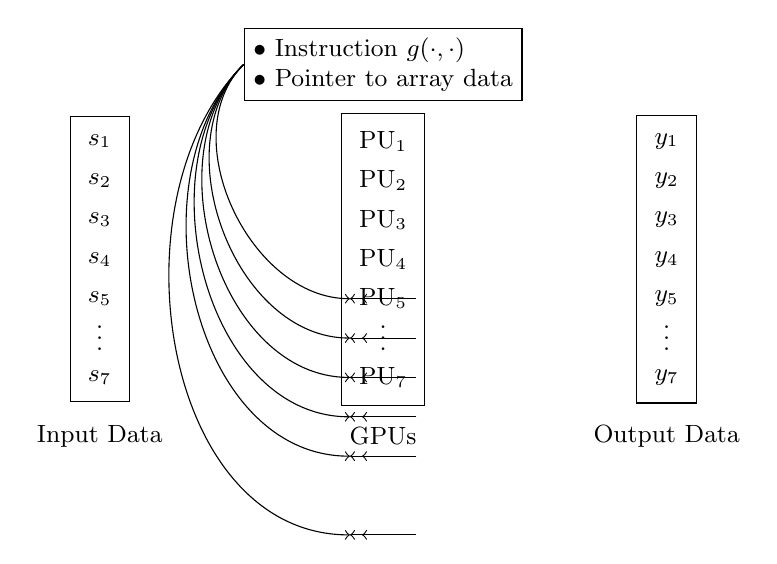
\begin{tikzpicture}[remember picture, scale=.9, font=\small]
            \node[draw,align=left] (I) at (0,2.75) {
              $\bullet$ Instruction $g(\cdot,\cdot)$\\
              $\bullet$ Pointer to array data
            };
            \node[draw] at (-4,0) {
              \tikz{
                \foreach\x in {1,2,3,4,5,7}{
                  \node (A\x) at (0,-\x/2) {$s_{\x}$};
                }
                \node at (0,-2.9) {$\vdots$};
              }
            };
            \node[draw] at (0,0) {
              \tikz{
                \foreach\x in {1,2,3,4,5,7}{
                  \node (B\x) at (0,-\x/2) {$\text{PU}_{\x}$};
                }
                \node at (0,-2.9) {$\vdots$};
              }
            };
            \node[draw] at (4,0) {
              \tikz{
                \foreach\x in {1,2,3,4,5,7}{
                  \node (C\x) at (0,-\x/2) {$y_{\x}$};
                }
                \node at (0,-2.9) {$\vdots$};
              }
            };
            \foreach\x in {1,2,3,4,5,7}{
              \draw[->] (A\x.east) -- (B\x.west);
              \draw[->] (B\x.east) -- (C\x.west);
              \draw[->] (I.west) to [out=-135,in=180] (B\x.west);
            }
            \node at (-4,-2.5) {Input Data};
            \node[align=center] at (0,-2.5) {GPUs};
            \node at (4,-2.5) {Output Data};
          \end{tikzpicture}
        }
      }
      \scalebox{.75}{
        \visible<2->{
          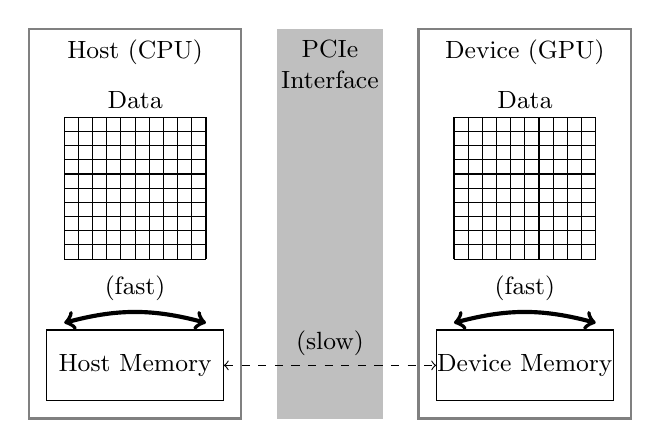
\begin{tikzpicture}[remember picture, scale=.9, font=\small]

            \fill[lightgray] (3.25,-.75) rectangle (4.75,4.75) node[black,midway,align=center,yshift=57.5] {PCIe\\Interface};
            \draw[gray,thick] (-.25,-.75) rectangle (2.75,4.75) node[black,midway,align=center,yshift=62] {Host (CPU)};
            \draw[gray,thick] (5.25,-.75) rectangle (8.25,4.75) node[black,midway,align=center,yshift=62] {Device (GPU)};

            \node[align=center] at (1.25, 3.75) {Data};
            \node[align=center] at (6.75, 3.75) {Data};

            % Host Memory
            \draw (0,-.5) rectangle (2.5,.5) node[midway] {Host Memory};

            % Device Memory
            \draw (5.5,-.5) rectangle (8,.5) node[midway] {Device Memory};


            % Arrow with Dashed Line
            \draw[<->, dashed] (2.5, 0) -- (5.5, 0) node[midway, above, align=center] {(slow)};
            \draw[<->, line width=1.5] (.25, .6) to [in=165, out =15] node[midway, above, align=center] {(fast)}(2.25, .6) ;
            \draw[<->, line width=1.5] (5.75, .6) to [in=165, out =15] node[midway, above, align=center] {(fast)}(7.75, .6) ;

            \def\rows{10}
            \def\cols{10}
            \def\elementwidth{2}
            \foreach \xshift/\yshift in {.25/1.5, 5.75/1.5} {
              % Draw Grid
              \foreach \i in {0,...,\rows} {
                \draw (\xshift, \yshift+\i*\elementwidth/\rows) -- (\xshift+\elementwidth, \yshift+\i*\elementwidth/\rows);
              }
              \foreach \i in {0,...,\cols} {
                \draw (\xshift+\i*\elementwidth/\cols, \yshift) -- (\xshift+\i*\elementwidth/\cols, \yshift+\elementwidth);
              }
            }
          \end{tikzpicture}
        }
      }
    \end{center}
    % \item Particularly efficient for dense matrix-matrix multiplication.
  \item<3-> To achieve optimal performance, all data should {\bf reside exclusively on device memory}.
  \item<4-> Heterogeneous architectures due to {\bf various hardware vendors} (NVIDIA, AMD, and Intel).
  \end{itemize}
  \visible<5>{
    \begin{center}
      \tikz{
        \node[rounded corners, fill=black!10,text width=.95\textwidth,align=center,inner sep=5] at (0,0) {
          Adapting CPU algorithms into GPU algorithms is \textbf{not merely a matter of software engineering} and often requires a \textbf{complete redesign of the algorithm}.
        };
      }
    \end{center}
  }
\end{frame}

\begin{frame}{Exascale Computing Project}
  \begin{itemize}
  \item {\bf Mission}: Harness exascale computing capabilities to tackle {\bf real-world challenges}.
    \begin{center}
      \begin{tikzpicture}[font=\scriptsize,align=center]
        \node at (-4,0) {\includegraphics[width=2.5in]{national-labs.png}};
        \node at (2.25,.9) {
          {\bf Frontier} @Oak Ridge (AMD GPUs)\\
          \includegraphics[height=.6in]{frontier.png}
        };
        \node at (2.25,-.9) {
          {\bf Aurora} @Argonne (Intel GPUs)\\
          \includegraphics[height=.6in]{aurora.jpg}
        };
      \end{tikzpicture}
    \end{center}
  \item<2-> {\bf Challenge}: There were no implementations of {\bf sparse automatic differentiation, nonlinear optimization solver, nor sparse indefinite solvers} on GPUs.
  \item<3-> {\bf Goal}: Build a {\bf comprehensive software infrastructure} for nonlinear optimization on GPUs.
    \begin{itemize}
    \item {\bf Performance}: at least an order of magnitude speedup.
    \item {\bf Portability}: compatibility with NVIDIA, AMD, and Intel.
    \item {\bf Application}: energy infrastructure problems.
    \end{itemize}
  \end{itemize}
\end{frame}

\begin{frame}{Language of Choice: Julia}
  \begin{itemize}
  \item Julia resolves the ``{\bf two-language problem}''; we're experiencing 10x faster development.
  \item<2-> {\bf Multiple dispatch}: High-level abstraction while specializing for specific data types.
  \item<3-> {\bf Portable programming}: Compatibility across various architectures (NVIDIA, AMD, Intel, etc.)
  \item<4-> {\bf JIT compilation}: No performance compromises, running as fast as C/C++/Fortran.
  \item<5-> The initial delay, often referred to as ``{\bf time-to-first-call},'' has been significantly reduced.
  \end{itemize}
  \begin{center} 
    \visible<4->{
      \includegraphics[height=1.75in]{speed-comparison.png}
    }
    \visible<5->{
      \includegraphics[height=1.75in]{TTFP.pdf}
    }
  \end{center}
\end{frame}


\begin{frame}{Summary of Exanauts' Journey}
  \begin{center}
    \begin{tikzpicture}[looseness=1,overlay, remember picture, xshift=-50]
      \draw[-latex,dashed] (-4,0) to (-4.5,-2) to (-1,-4) to (.5,2) to (-.5,0) to (-1.5,-3) to (-.5,2) to (-2.5,1) to (-3,0) to (0,0);
      \draw[-latex] (-4,0) -- (0,0);

      \draw[-latex] (-5,-3.6) -- ++ (.5,0) node[right,anchor=west,font=\scriptsize] {Ideal Research Progres};
      \draw[-latex,dashed] (-5,-4) -- ++(.5,0) node[right,anchor=west,font=\scriptsize] {Our Journey};
      \visible<2->{
        \node[align=left, text width=.5\textwidth] at (5.5,-.5) {
          \begin{itemize}
          \item {\bf Nonlinear optimization/linear algebra}:\\
            distributed Jacobi, Lagrangian decomposition, ADMM, batched TRON solver, domain decomposition preconditioners, 
            \only<2>{reduced-space interior point method, condensed interior-point methods w/ inequality relaxation}\only<3>{{\color{blue}reduced-space interior point method, condensed interior-point methods w/ inequality relaxation}}, ...
          \item {\bf Modeling/automatic differentiation}:\\
            batched second-order adjoint sensitivity,
            \only<2>{SIMD abstraction}\only<3>{{\color{blue}SIMD abstraction}}, ...
          \item {\bf Packages developed}:\\
            ExaPf, Argos, ExaADMM, BlockPowerFlow, ProxAL, ExaTron, \only<2>{MadNLP, ExaModels}\only<3>{{\color{blue}MadNLP, ExaModels}}, ...
          \end{itemize}
        };
      }
    \end{tikzpicture} 
  \end{center}
  \reference{
    M. Anitescu et. al. {\it Targeting Exascale with Julia on GPUs for multiperiod optimization with scenario constraints}. SIAG/OPT Views and News (2021).
  }
\end{frame}

\begin{frame}{Two Award-Winning Open-Source Projects {\small (2023 COIN-OR Cup)}}
  \begin{center}
    \begin{tikzpicture}[remember picture,overlay,align=center] 
      \node at (-3.75,1) {
        \includegraphics[width=2.75in]{examodels.pdf}
      };
      \node at (3.75,1) {
        \includegraphics[width=2.75in]{madnlp.pdf}
      };
      \node at (-4,-.5) {
        \footnotesize\url{https://github.com/sshin23/ExaModels.jl}
      }; 
      \node at (4,-.5) {
        \footnotesize\url{https://github.com/MadNLP/MadNLP.jl}
      };
      \node at (0, -2.5) {
        \includegraphics[height=2cm]{shin.jpg}
        \includegraphics[height=2cm]{pacaud.jpg}
        \includegraphics[height=2cm]{anitescu.jpg}
        \includegraphics[height=2cm]{coin-or.png} 
      };
    \end{tikzpicture}
  \end{center}
\end{frame}
 

\begin{frame}{How \{AMPL, IPOPT, Ma27\} Have Succeeded on CPUs}
  \centering
  \begin{tikzpicture}[align=center,font=\footnotesize,overlay, remember picture] 
    \node[rounded corners, fill=black!10, text width=.225\textwidth, minimum height=.2\textheight] (A1) at (-5.7,2) {      
      \begin{align*}
        \min_{x\geq 0}\;& f(x)\\
        \st\;& c(x) = 0
      \end{align*}      
    };
    \node[rounded corners, fill=black!10, text width=.225\textwidth, minimum height=.2\textheight] (A2) at (-1.9,2) {      
      \begin{align*}
        \min_{x}\;& f(x) - \mu \log(x)\\
        \st\;& c(x) = 0
      \end{align*}
      
    };
    \node[rounded corners, fill=black!10, text width=.225\textwidth, minimum height=.2\textheight,font=\scriptsize] (A3) at (1.9,2) {      
      \begin{align*}
        \hspace{-.5em}
        \setlength\arraycolsep{2pt}
        \underbrace{\begin{bmatrix}
          W + \Sigma +\delta_w I& A^\top\\
          A & \delta_c I
        \end{bmatrix}
              \hspace{-.5em}
              \begin{bmatrix}
                \Delta x\\ \Delta \lambda
              \end{bmatrix}
        \hspace{-.25em} 
        =
        \hspace{-.25em}
        \begin{bmatrix}
          p^x\\p^\lambda
        \end{bmatrix}}_{\text{\scriptsize "KKT System"}}
      \end{align*}      
    };
    \node[rounded corners, fill=black!10, text width=.225\textwidth, minimum height=.2\textheight] (A4) at (5.7,2) {
      \begin{align*}
        x^{(k+1)}  = x^{(k)} + \alpha \Delta x\\
        \lambda^{(k+1)}  = \lambda^{(k)} + \alpha \Delta \lambda 
      \end{align*}      
    };
    \node[font=\footnotesize\bf] at (-5.7,2.65) {Modeling};
    \node[font=\footnotesize\bf] at (-1.9,2.65) {Barrier Reformulation};
    \node[font=\footnotesize\bf] at (1.9,2.65) {Newton's Step Comp.};
    \node[font=\footnotesize\bf] at (5.7,2.65) {Line Search};

    \only<2->{
      \node[font=\footnotesize,text width=.3\textwidth,fill=red!10,rounded corners] (B1) at (-5,-.5) {
        {\bf Algebraic Modeling Systems}\\[.5em]
        AMPL, JuMP, CasADi, ...
      };
    }
    \only<3->{
      \node[font=\footnotesize,text width=.3\textwidth,fill=blue!10,rounded corners] (B2) at (0,-.5) {
        {\bf Nonlinear Optimization Solvers}\\[.5em]
        Ipopt, Knitro, Pynumero, ...
      };
    }
    \only<4->{
      \node[font=\footnotesize,text width=.3\textwidth,fill=green!10,rounded corners] (B3) at (5,-.5) {
        {\bf Sparse Linear Solvers}\\[.5em]
        HSL (ma27, ma57, ...), Pardiso, ...
      }; 
    }
    \only<2->{
      \draw[red,latex-] (A1.south) -- (B1.north);
      \draw[red,latex-] (A3.south) -- (B1.north);
    }
    \only<3->{
      \draw[blue,latex-] (A2.south) -- (B2.north);
      \draw[blue,latex-] (A3.south) -- (B2.north);
      \draw[blue,latex-] (A4.south) -- (B2.north);
    }
    \only<4->{
      \draw[ForestGreen,latex-] (A3.south) -- (B3.north);
    }
    \node[text width=\textwidth,font=\normalsize] at (0,-2.5) {
      \begin{itemize}
      \item<2-> Algebraic modeling systems have enabled efficient {\bf sparse automatic differentiation}.
      \item<3-> Interior-point solvers have removed the combinatorial complexities of inequality constraints; however, we pay the price by solving {\bf extremely ill-conditioned linear systems}.
      \item<4-> Sparse indefinite solvers have enabled {\bf the solution of ill-conditioned linear systems}. 
      \end{itemize}
    };
  \end{tikzpicture}
\end{frame}

\begin{frame}{Why it is Challenging: Sparse Automatic Differentiation} 
  \begin{itemize}
  \item {\bf Automatic differentiation} is {\bf more efficient} than {\it finite difference} or {\it symbolic differentiation}, and is {\bf less prone to error} than {\it hand-written derivative codes}.
    \begin{center}
      \vspace{.2in}
      \begin{tikzpicture}[overlay, remember picture] 
        \node[rounded corners,fill=red!10,minimum width=1.5in] (1) at (-4,0) {\tt f(x)\{ ... \}};
        \node[rounded corners,fill=red!10,minimum width=1.5in] (2) at (4,0) {\tt df(x)\{ ... \}};
        \node[rounded corners,fill=blue!10,minimum width=1.5in] (3) at (-4,-2) {$y=f(x)$};
        \node[rounded corners,fill=blue!10,minimum width=1.5in] (4) at (4,-2) {$y'=f'(x)$};
        \only<5->{
          \draw[-latex,font=\footnotesize\it] (1) -- node[above] {Automatic Differentiation} node[below] {(e.g., AMPL, JuMP, Torch)} (2);
        }
        \only<3->{
          \draw[-latex,font=\footnotesize\it, dashed] (3) -- node[above] {Symbolic Differentiation} node [below] {(e.g., Mathematica, Maple)} (4);
          \draw[-latex,font=\footnotesize\it, dashed] (1) -- (3);
          \draw[latex-,font=\footnotesize\it, dashed] (2) -- (4);
        }
        \only<2->{
          \draw[latex-,font=\footnotesize\it] (1.south) -- ++ (-.75,-.75) node[anchor=east] {Finite Difference} ;
        }
        \only<4->{
          \draw[latex-,font=\footnotesize\it] (2.south) -- ++ (-.75,-.75) node[anchor=east] {Hand-Written Derivative Code};
        }
      \end{tikzpicture}
      \vspace{1.1in}
    \end{center}
  \item<6-> Existing {\bf algebraic modeling systems} (e.g., AMPL and JuMP) are {\bf designed for CPUs}.
  \item<7-> {\bf Machine learning frameworks} (e.g., Torch) are not effective for {\bf sparse problems}.
  \end{itemize}
\end{frame}

\begin{frame}{Solution: SIMD Abstraction}
  \begin{itemize}
  \item<1-> Large-scale optimization problems {\bf almost always have repetitive patterns}.\\
    e.g., optimal power flow w/ millions of variables can be expressed with a handful of patterns.
    \vspace{-.15in}
    \begin{columns}[t]
      \footnotesize
      \begin{column}{0\textwidth}
      \end{column}
      \begin{column}{.3\textwidth}
        \begin{itemize}
        \item referencebus voltage angle
          \vspace{-.05in}
        \item active and reactive power flow
        \end{itemize}
      \end{column}
      \begin{column}{.3\textwidth}        
        \begin{itemize}
        \item voltage angle difference limits
          \vspace{-.05in}
        \item apparent power flow limits
        \end{itemize}
      \end{column}
      \begin{column}{.3\textwidth}        
        \begin{itemize}
        \item generation cost
          \vspace{-.05in}
        \item power balance equations
        \end{itemize}
      \end{column}
    \end{columns}
    \visible<2->{
      \begin{align*}
        \min_{x^\flat\leq x \leq x^\sharp}
        & \sum_{l\in[L]}\sum_{i\in [I_l]} f^{(l)}(x; p^{(l)}_i)\tag{\bf SIMD abstraction}\\
        \st\;
        &
          \left[g^{(m)}(x; q_j)\right]_{j\in [J_m]} +\sum_{n\in [N_m]}\sum_{k\in [K_n]}h^{(n)}(x; s^{(n)}_{k}) =0, \quad \forall m\in[M]
      \end{align*}
    }
    \vspace{-.1in} 
  \item<3-> Repeated patterns are made available by always specifying the models as {\bf iterable objects}.
    \begin{center}
      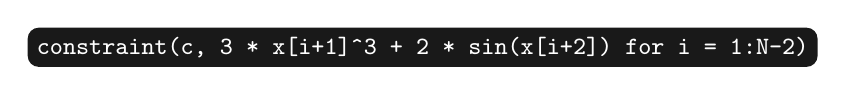
\begin{tikzpicture}
        \node[rounded corners, fill=black!90, font=\color{white}\small] at (0,0) {\tt
          constraint(c, 3 * x[i+1]\^{}3 + 2 * sin(x[i+2]) for i = 1:N-2)
        };
      \end{tikzpicture}
    \end{center} 
  \item<4-> {\bf For each repeatitive pattern}, the derivative evaluation kernel is constructed \& compiled,\\ and it is {\bf executed in parallel over multiple data}.
  \end{itemize}
  \reference{
    S. Shin, F. Pacaud, and M. Anitescu. {\it Accelerating optimal power flow with GPUs: SIMD abstraction of nonlinear programs and condensed-space interior-point methods}, arXiv:2307.16830.
  }
\end{frame}

\begin{frame}{Why it is Challenging: Sparse Linear Solvers}
  \begin{itemize}
  \item<1-> Solving KKT systems on CPUs has traditionally relied on {\bf direct LBL$^\top$ factorization}.
    \begin{center}
      \tikz{
        \node[inner sep=0pt] (augmented) at (-4,0) {\includegraphics[width=1.25in]{augmented.pdf}};
        \node[inner sep=0pt] (facL) at (0,0) {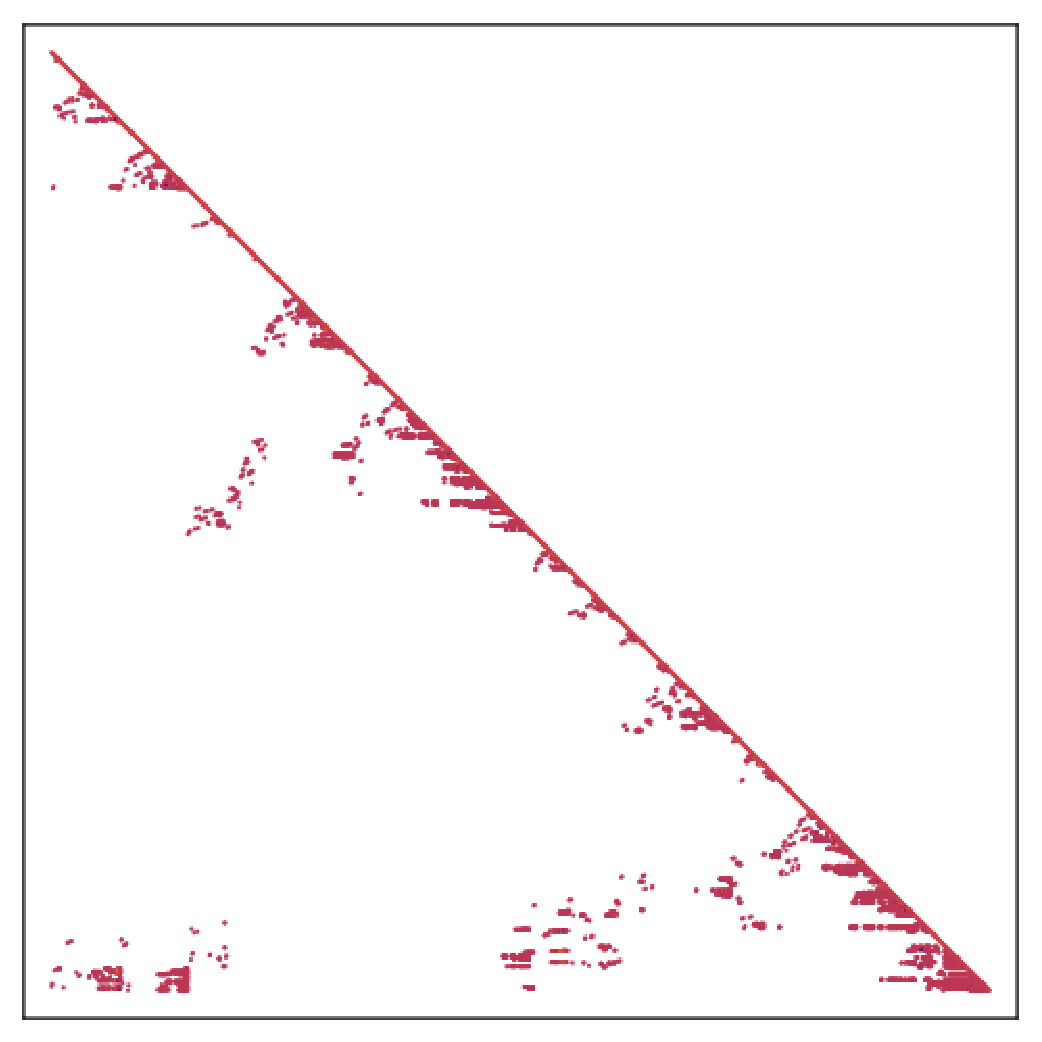
\includegraphics[width=1.25in]{lu_L.pdf}};
        \node[inner sep=0pt] (facU) at (6,0) {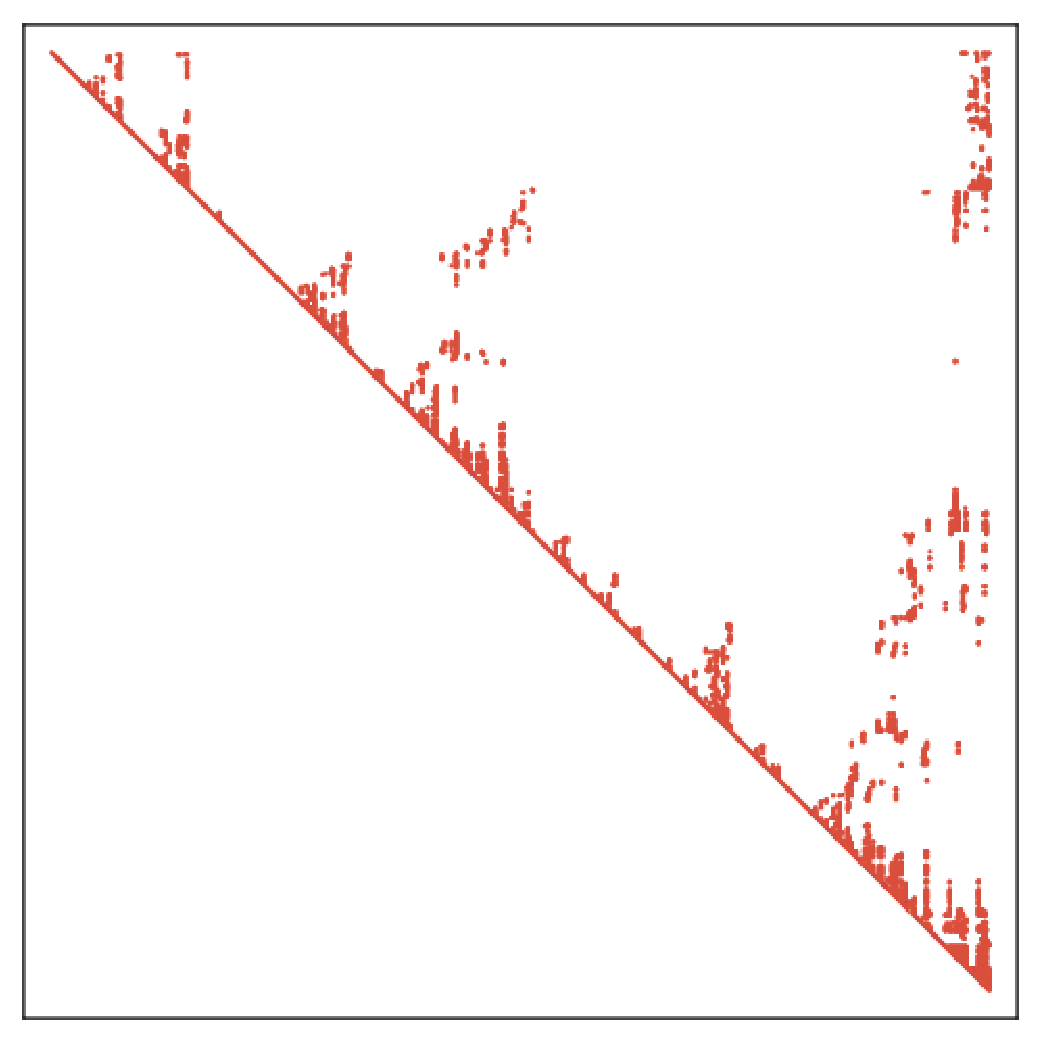
\includegraphics[width=1.25in]{lu_U.pdf}};
        \node[inner sep=0pt] at ($(facL)!.5!(augmented)$) {$=$};
        \node[inner sep=0pt] at ($(facL)!.35!(facU)$) {$\times$};
        \node[inner sep=0pt] at ($(facL)!.65!(facU)$) {$\times$};
        \node[align=center,inner sep=0pt,yshift=-12] at ($(facL)!.5!(facU)$) {$B$\\\footnotesize (1x1 or 2x2\\[-.25em]\footnotesize block-diagonal)};
      } 
    \end{center}
  \item<2-> Achieving numerical stability necessitates {\bf numerical pivoting}, a process that is notoriously {\bf challenging to parallelize}.
  \item<3-> Due to the ill-conditioning of the KKT system, {\bf iterative methods} are generally impractical, although there have been some promising results with {\bf specialized preconditioners}.
  \end{itemize}
  \visible<3->{
    \reference{
      Curtis, Huber, Schenk, Waechter. {\it A note on the implementation of an interior-point algorithm for nonlinear optimization with inexact step computations}. MathProg. (2012)\\
      Cao, Seth, Laird. {\it An augmented Lagrangian interior-point approach for large-scale NLP problems on graphics processing units}. CACE. (2016)\\
      Gondzio, Matrix-free interior point method, Comput Optim Appl (2012)
    }
  }
\end{frame}

\begin{frame}{Solution \#1: Condensed-Space Interior Point Method} 
  \begin{itemize}
  \item<1-> We aim to transform the KKT systems into a {\bf sparse positive definite system}.
  \item<2-> Can be achieved by (i) converting the {\bf equalities into inequalities}:
    \begin{align*}
      g(x) = 0 \quad\Longrightarrow\quad g(x)- s = 0,\quad s^{\flat}\leq s\leq  s^\sharp,
    \end{align*}
    \visible<3->{
      (ii) {\bf eliminating the slack variables} (so-called {\it condensation}):
      \begin{align*}\scriptsize
        \begin{bmatrix}
          W^{(\ell)}  + \delta^{(\ell)}_w I & & A^{(\ell)\top}& -I & I &  \\
          & \delta^{(\ell)}_w I & -I&&&-I & I\\
          A^{(\ell)}& -I & -\delta^{(\ell)}_c I\\
          Z_x^{(\ell)\flat}&&&X^{(\ell)}-X^\flat\\
          -Z_x^{(\ell)\sharp}&&&&X^\sharp-X^{(\ell)}\\
          &Z_s^{(\ell)\flat}&&&&S^{(\ell)}-S^\flat\\
          &-Z_s^{(\ell)\sharp}&&&&&S^\sharp-S^{(\ell)}\\
        \end{bmatrix}
        \begin{bmatrix}
          \Delta x \\
          \Delta s \\
          \Delta y \\
          \Delta z_x^\flat \\
          \Delta z_x^\sharp \\
          \Delta z_s^\flat \\
          \Delta z_s^\sharp \\
        \end{bmatrix} =
        \begin{bmatrix}
          p^{(\ell)}_{x }\\
          p^{(\ell)}_{s }\\
          p^{(\ell)}_{y }\\
          p^{(\ell)}_{z_x^\flat }\\
          p^{(\ell)}_{z_x^\sharp }\\
          p^{(\ell)}_{z_s^\flat }\\
          p^{(\ell)}_{z_s^\sharp }\\
        \end{bmatrix}\\
        \Longrightarrow\quad
        \color{blue}{(W + \delta_wI + \Sigma_x + A^{\top} D A ) \Delta x = q_x + A^\top (C q_s +  Dq_y )}
      \end{align*}
    }
    \vspace{-.2in}
  \item<4-> These systems can be solved {\bf without numerical pivoting} (routines available in CUDA).
  \end{itemize}
  \reference{
    S. Shin, F. Pacaud, and M. Anitescu. {\it Accelerating optimal power flow with GPUs: SIMD abstraction of nonlinear programs and condensed-space interior-point methods}, arXiv:2307.16830.
  }
\end{frame}

\begin{frame}{Solution \#2: Reduction \& Dense Reformulation} 
  \begin{itemize}
  \item<1-> Oftentimes, the decision variables can be {\bf splitted into state} and {\bf control variables}.
  \item<2-> We {\bf reduce the KKT systems} by {\bf elimintating the state variables} [Biegler, 1995].
  \item<3-> This {\bf reduction} transforms the KKT system into a compact, dense, positive definite system.
    \begin{center}
      \begin{tikzpicture}[font=\footnotesize\bf]
        \node at (0,0) {\includegraphics[width=.7\textwidth]{reduction.png}};
        \node at (-3.7,2) {Original};
        \node at (0,2) {Condensed};
        \node at (3.7,2) {Condensed \& Reduced};
      \end{tikzpicture}      
    \end{center}
  \item<4-> {\bf The elimination is a bottleneck}, but can be accelerated by exploiting structures\\
    (e.g., Riccati recursion for optimal control).
  \end{itemize}
  \reference{
    L. Biegler, J. Nocedal, C. Schmid. {\it A reduced Hessian method for large-scale constrained optimization}. SIOPT (1995).\\
    F. Pacaud, S. Shin, M. Schanen, D. A. Maldonado, and M. Anitescu. {\it Accelerating condensed interior-point methods on SIMD/GPU architectures}. JOTA (2023). \\
    D. Cole, S. Shin, F. Pacaud, V. M. Zavala, and M. Anitescu. {\it Exploiting GPU/SIMD architectures for solving linear-quadratic MPC problems}. ACC (2023).
  }
\end{frame}


\begin{frame}{Highlight: AC Optimal Power Flow {\normalsize (single GPU)}}
  \begin{itemize}
  \item<1-> Standard form polar form AC optimal power flow (AC OPF) problems.
  \item<1-> The condensed-space interior point method is employed.
  \item<1-> Solved up to $10^{-4}$ precision (note that by default, Ipopt solves up to $10^{-8}$ precision).
  \item<2-> For large-scale cases, GPU becomes {\bf significantly faster than CPU } \visible<3->{{\color{blue}(up to $\times 10$ speedup).}}
    \vspace{.1in}
    \begin{center}
      \scriptsize
      \begin{tabular}{|l|c|c|ccc|ccc|}
  \hline
  \multirow{3}{*}{\textbf{Case}}
  & \multirow{3}{*}{\# vars}
  & \multirow{3}{*}{\# cons}
  & \multicolumn{3}{c|}{\textbf{MadNLP+ExaModels+cuSOLVER}}
  & \multicolumn{3}{c|}{\textbf{Ipopt+AMPL+Ma27}}
  \\
  & & &\multicolumn{3}{c|}{\textbf{(GPU$^*$)}} &\multicolumn{3}{c|}{\textbf{(CPU$^{**}$)}}
  \\
  \cline{4-9}
  & & 
  & \quad \# iter \quad& \quad AD$^\dag$  \quad&  \quad total$^\dag$ \quad
    & \quad \# iter \quad& \quad AD$^\dag$  \quad&  \quad total$^\dag$ \quad
  \\
  \hline
  10480\_goc 
  &  96.8k
  & 150.9k
  & 70 
  &  0.13
  & 14.26
    & 64 
      & 16.93
                                               & 38.04
  \\

  13659\_pegase 
  & 117.4k
  & 170.6k
  & 63 
  &  0.12
  &  7.15
    & 64 
      & 19.70
                                               & 35.66
  \\

  19402\_goc 
  & 179.6k
  & 281.7k
  & 79 
  &  0.17
  & 23.28
    & 70 
      & 36.50
                                               & 95.34
  \\

  24464\_goc 
  & 203.4k
  & 313.6k
  & 63 
  &  0.11
  & 70.63
    & 58 
      & 33.50
                                               & 70.15
  \\

  30000\_goc 
  & 208.6k
  & 307.8k
  & 162 
  &  0.33
  & 22.05
    & 180 
      & 101.98
                                               & 249.81
  \\
    \hline  
\end{tabular}\\
      AD = Automatic Differentiation\\
      $^\dag$Wall time (sec) measured by Julia. $^\ddag$CPU time (sec) reported by Ipopt.\\
      $^*$NVIDIA Quadro GV100  $^{**}$Intel Xeon Gold 6140
    \end{center}
  \item<4-> Automatic differentiation is $\times 300$ faster, and the rest of computation is $\times 8$ faster. 
  \end{itemize}
  \reference{
    S. Shin, F. Pacaud, and M. Anitescu. {\it Accelerating optimal power flow with GPUs: SIMD abstraction of nonlinear programs and condensed-space interior-point methods}, arXiv:2307.16830.
  }
\end{frame}

\begin{frame}{Highlight: Security-Constrained AC OPF {\normalsize (multi GPU)}}
  \begin{itemize}
  \item<1-> Standard security-constrained AC optimal power flow (SC AC OPF) problems.
  \item<1-> The {\bf reduction \& dense formulation} and the {\bf classical Schur-complement method for block-structured problems} are employed.
  \item<2-> Leveraging {\bf multiple GPUs} allows us to {\bf overcome the limitations} of a single GPU.
    \vspace{.1in}
    \begin{center}
      \scriptsize
      \begin{tabular}{|l|cccc|cccc|cccc|}
  \hline
  &
    \multicolumn{4}{c|}{\bf 1354pegase}
  &
    \multicolumn{4}{c|}{\bf 2869pegase}
  &
    \multicolumn{4}{c|}{\bf 9241pegase} \\
  \hline
  &
    \# iter
  & AD
  & LA
  & total
  &
    \# iter
  & AD
  & LA
  & total
  &
    \# iter
  & AD
  & LA
  & total \\
  \hline
  {\bf CPU$^{*}$}
  &
    44
  & 2.6
  & 4.2
  & {7.0}
  &
    77
  & 11.9
  & 27.4
  & {40.3}
  &
    136
  & 205.6
  & 771.8
  & {984.1} \\
  {\bf 1 GPU$^{**}$}
  &
    44
  & 0.3
  & 1.8
  & {2.1}
  &
    93
  & 1.1
  & 11.7
  & {12.8}
  &
    98
  & 5.5
  & 112.3
  & {117.8}\\
  {\bf 2 GPUs$^{**}$}
  &
    44
  & 0.3
  & 1.1
  & {1.4}
  &
    93
  & 0.8
  & 7.4
  & {8.2}
  &
    98
  & 3.4
  & 56.8
  & {60.2}\\
  {\bf 4 GPUs$^{**}$}
  &
    44
  & 0.3
  & 1.0
  & {1.3}
  &
    93
  & 0.8
  & 5.7
  & {6.5}
  &
    98
  & 2.3
  & 35.8
  & {38.1}\\
  {\bf 8 GPUs$^{**}$}
  &
    44
  & 0.2
  & 1.0
  & {1.2}
  &
    93
  & 0.6
  & 5.1
  & {5.7}
  &
    98
  & 1.4
  & 26.4
  & {27.7}\\
  \hline
  {\bf \# vars} & \multicolumn{4}{c|}{20k} & \multicolumn{4}{c|}{42k} & \multicolumn{4}{c|}{139k}\\
  {\bf \# cons} & \multicolumn{4}{c|}{53k} & \multicolumn{4}{c|}{119k} & \multicolumn{4}{c|}{404k}\\
  \hline
\end{tabular}\\
      AD = Automatic Differentiation, LA = Linear Algebra (KKT System Solver)\\
      $^{*}$AMD CPU Epyc ”Milan” $^{**}$NVIDIA A100 (4 GPUs per node) 
    \end{center}
  \end{itemize}
  \reference{
    F. Pacaud, M. Schanen, S. Shin, D. A. Maldonado, and M. Anitescu. {\it Parallel interior-point solver for block-structured nonlinear programs on SIMD/GPU architectures}. arXiv:2301.04869.
  }
\end{frame}

\begin{frame}{Highlight: Security-Constrained AC OPF {\normalsize (multi GPU)}}
  \vspace{.1in} 
  \begin{itemize}
  \item<1-> Our approach is $\times 6$ faster than commercial multi-CPU solver.
    \begin{center}
      \includegraphics[height=.45\textheight]{kkt_timings.pdf}
    \end{center}
  \item<2-> Single-node, multi-GPU parallelism is more efficient than multi-node, multi-GPU.
    \begin{center}
      \includegraphics[height=.3\textheight]{nvlink.png}
    \end{center}
  \end{itemize}
  \reference{
    F. Pacaud, M. Schanen, S. Shin, D. A. Maldonado, and M. Anitescu. {\it Parallel interior-point solver for block-structured nonlinear programs on SIMD/GPU architectures}. arXiv:2301.04869.
  }
\end{frame}

% \begin{frame}{On-going Works}
%   \begin{itemize}
%   \item Other projects: HiOp (HPC nonlinear optimization solver) and HyKKT (KKT system solver)
%   \item Running nonlinear optimization on Frontier (AMD GPUs) and Aurora (Intel GPUs).
%   \item Preconditioned iterative methods for solving KKT systems.
%   \item Specialzied solvers for nonlinear optimal control.
%   \item Have an idea? Happy to chat!
%   \end{itemize}
% \end{frame}

\begin{frame}{Conclusions}
\begin{itemize}
  \item Modern GPU hardware offers significant potential for accelerating large-scale optimization.
  \item Implementing algorithms on GPUs can be challenging and often {\bf requires reevaluating key aspects of existing algorithms}.
  \item We have achieved promising results: up to \textbf{10x faster solutions with moderate accuracy}, though challenges remain for high-accuracy solutions.
  \item GPU-based optimization opens up opportunities to address previously intractable problems:
    \begin{itemize}
    \item {\bf Extremely large-scale} problems (multi-stage, multiscale).
    \item Problems involving {\bf expensive surrogate models} (neural nets, simulations).
    \end{itemize}
  \end{itemize}
  \visible<2->{
    \begin{center}
      \tikz{
        \node[rounded corners, fill=red!10,text width=.85\textwidth,align=center,inner sep=5] at (0,0) {
          {\bf Shin Group @ MIT is hiring postdocs}! Find more details here:\\ 
          \url{https://shin.mit.edu}
        };
      }
    \end{center}
  }
\end{frame}

\begin{frame}{Acknowledgement}
  \nocite{shin2022accelerating}
  \nocite{pacaud2023parallel} 
  \nocite{pacaud2023accelerating}
  \nocite{anitescu2021targeting}
  \begin{center}
    \tikz[align=center,font=\footnotesize]{
      \node at (0,0) {
        \bf U.S. Department of Energy, Office of Science, \\
        \bf Advanced Scientific Computing Research\\
        (DE-AC02-06CH11347)
      };
      \node at (7,0) {
        \bf U.S. Department of Energy, Office of Science\\
        \bf and National Nuclear Security Administration,\\
        {\bf Exascale Computing Porject} (17-SC-20-SC)
      };
      \node at (0,-1.5) {
        \includegraphics[height=.2\textheight]{doe.png}
      };
      \node at (7,-1.5) {
        \includegraphics[height=.2\textheight]{ecp.png}
      };
    }
  \end{center}
  {
    \footnotesize
    \bibliography{main}
  }
\end{frame}


\begin{frame}[noframenumbering,plain]
  \mytitlepage
\end{frame}

\end{document}